\begin{figure}[H]
		\centering
		
		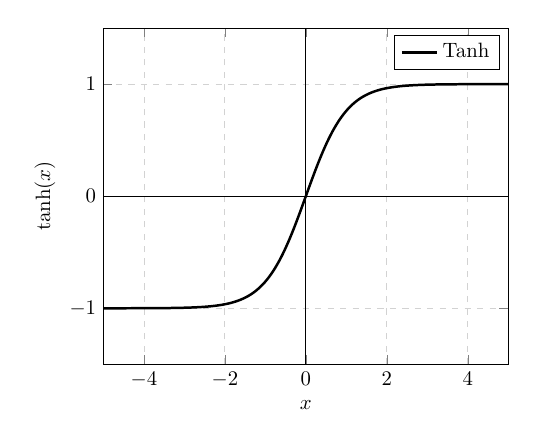
\begin{tikzpicture}[scale=0.75]
			\begin{axis}[
				xlabel=$x$, ylabel=$\tanh(x)$,
				xmin=-5, xmax=5,
				ymin=-1.5, ymax=1.5,
				grid=major, grid style={dashed, gray!35},
			]
			\addplot[black, samples=500, very thick] {tanh(x)};
			
			% This plots a horizontal line from xmin to xmax
			\draw[semithick] (axis cs:\pgfkeysvalueof{/pgfplots/xmin}, 0) -- (axis cs:\pgfkeysvalueof{/pgfplots/xmax}, 0);
			
			% This plots a vertical line from ymin to ymax
			\draw[semithick] (axis cs:0, \pgfkeysvalueof{/pgfplots/ymin}) -- (axis cs:0, \pgfkeysvalueof{/pgfplots/ymax});
			
			\addlegendentry{Tanh}
			\end{axis}
		\end{tikzpicture}
		
		\caption{Hyperbolic tangent activation function.}
		\label{fig:tanh}
	\end{figure}